\documentclass[conference]{IEEEtran}
\IEEEoverridecommandlockouts
% The preceding line is only needed to identify funding in the first footnote. If that is unneeded, please comment it out.
\usepackage{cite}
\usepackage{amsmath,amssymb,amsfonts}
\usepackage{algorithmic}
\usepackage{graphicx}
\usepackage{textcomp}
\usepackage{xcolor}
\usepackage{lipsum}
\usepackage{hyperref}
\usepackage{booktabs}
\hypersetup{colorlinks=true}
% ,urlcolor=blue,citecolor=black}
    % colorlink=blue,
    % linkcolor=blue
% }
\def\BibTeX{{\rm B\kern-.05em{\sc i\kern-.025em b}\kern-.08em
    T\kern-.1667em\lower.7ex\hbox{E}\kern-.125emX}}
    
\def\ColStyle#1{\textbf{\textit{#1}}}
\begin{document}

\title{Predicción de las Causas de los Incendios Forestales en EE.UU.}

\author{\IEEEauthorblockN{Francisco Muñoz Guajardo}
\IEEEauthorblockA{\textit{Departamento de Ingeniería Matemática} \\
\textit{Universidad de Chile, FCFM}
}
}

\maketitle

\begin{abstract}
En este informe se explorarán métodos para predecir las causas que producen un incendio dados algunos parámetros del mismo, como lo es el origen geográfico del incendio, la fecha en que ocurrió, la extensión del incendio, entre otras cosas.
\end{abstract}

% \begin{IEEEkeywords}
% component, formatting, style, styling, insert
% \end{IEEEkeywords}

\section{Introducción}

% Introducción breve, solo una pequeña introducción a su problema (contexto), resumen de lo realizado en presentación 1 y 2 y lo hecho para el informe final más el cumplimiento de los objetivos que tenían.

\subsection{Contexto y Motivación}
En el último tiempo se ha visto que han ocurrido un gran número de incendios en todo el mundo. Cómo lo es en el caso de Chile, el Amazonas (Brasil) o Australia. Es por esto, que se planteó en utilizar las herramientas de Aprendizaje de Máquinas para poder ayudar a combatir y prevenir los incendios que están aconteciendo.

En este trabajo se contará con un \textit{dataset} que cuenta con más de un millón y ochocientos mil incendios ocurridos en Estados Unidos de forma histórica. Una descripción más detallada acerca de los datos que se ocuparán se puede encontrar en \ref{descr-datos}.

\subsection{Preguntas realizadas}
Dadas algunas propiedades intrínsecas de un incendio, como lo es su ubicación geográfica, la fecha y hora de ocurrencia y algunos otros factores que se detallarán más adelante,
\begin{itemize}
    \item ¿Es posible predecir las causas de un incendio?
    \item ¿Es posible saber si un incendio es causado por error humano, por la naturaleza o con fines maliciosos?
\end{itemize}

\subsection{Objetivos}
Realizadas las preguntas a responder, se propondrán los siguientes objetivos:
\begin{itemize}
    \item Predecir las causas específicas de un incendio dados los datos que nos entrega el \textit{dataset}.
    \item Predecir las causas generales de un incendio dados los datos que nos entrega el \textit{dataset}.
\end{itemize}

\subsection{Resumen del trabajo realizado en la primera presentación}
En la primera presentación se empezó a buscar algún proyecto interesante, en el que se pueda aplicar las herramientas aprendidas en el curso. 

Escogido el tema, se plantearon las preguntas: ``\textit{¿Se puede predecir la extensión de un incendio?}'' Esta pregunta fue reemplazada con la pregunta ``\textit{¿Es posible predecir las causas de un incendio?}'' (se reemplazó pues se consideraba que para la primera pregunta se necesitan datos meteorológicos, los cuales no se cuenta actualmente).

Luego, se empezaron a buscar base de datos interesantes, de forma que pueda responder a las preguntas. Finalmente, se encontraron dos bases de datos: la correspondiente a los incendios de Estados Unidos (la cual se encuentra bastante detallada) y la correspondiente a la de CONAF, que es chilena. Finalmente, se prefirió la base de datos de Estados Unidos, pues la base de datos chilena tiene muy pocos datos, además de que solamente se encuentra disponible en Excel, dificultando su respectiva extracción de datos.

\subsection{Resumen del trabajo realizado en la segunda presentación}
En la segunda presentación, se seleccionaron las columnas que se consideraran relevantes de la base de datos de Estados Unidos. Paso siguiente, se empezó a preparar el \textit{dataset} para su posterior manipulación, eliminando algunos datos que no fueran importantes (como los datos faltantes o los datos duplicados), modificando el formato de los datos y agregando nuevas columnas al dataset.

Luego, se empezó realizando un análisis exploratorio de los datos, observando la distribución del número de incendios con respecto a las causas, a los estados (en el sentido de un estado de EE.UU.), a los días de la semana y con respecto a la hora. Luego se intentó observar la correlación entre las columnas.

Finalmente, se implementaron algunos modelos básicos ocupando la base de datos, como lo es \textit{Naïve Bayes}, \textit{K-Vecinos más Cercanos}, \textit{Random Forest}, entre otros.

\section{Descripción de los Datos} \label{descr-datos}

\subsection{Descripción preliminar de los datos}

Se cuenta con un \textit{dataset}, obtenido de \href{https://www.kaggle.com/rtatman/188-million-us-wildfires}{Kaggle}, con un registro de 1.880.465 incendios históricos ocurridos en Estados Unidos, desde 1992 hasta 2015. La información original se obtuvo a partir del \textit{U.S. Department of Agriculture} \cite{FPA}.

El \textit{dataset} se encuentra en extensión \textit{.sqlite}, de donde ocuparemos la tabla ``\textit{Fires}'', que posee en total 37 columnas, dentro de las cuales, existen columnas para describir el ID (como lo es \textit{\textbf{FOD\_ID}} O \textit{\textbf{FPA\_ID}}), las siglas (como lo es \textit{\textbf{STATE}}), los nombres (como lo es \textit{\textbf{SOURCE\_SYSTEM\_TYPE}}), algunos parámetros numéricos (como lo es \textit{\textbf{FIRE\_SIZE}}), parámetros temporales (como lo es \textit{\textbf{CONT\_DATE}} o \textit{\textbf{CONT\_TIME}}), parámetros espaciales (como lo es \textit{\textbf{LATITUDE}}), entre otros (que no viene al caso describir cada una de las columnas del \textit{dataset}, dado a que posee una cantidad abrumadora de columnas). Dentro de las cuales, la columna de etiquetas (que en nuestro caso viene a ser lo mismo que las causas) que se desea predecir es la llamada \textit{\textbf{STAT\_CAUSE\_DESCR}}.

Para más información acerca de las columnas del \textit{dataset}, se puede consultar la documentación proporcionada en la página de Kaggle.

\subsection{Descripción de las columnas a ocupar}

Del total de columnas que posee la tabla, ocuparemos aquellas que estén relacionadas con la fecha (como la hora y la fecha estimada en que se inició el incendio y el momento en que se controló), la geografía (como las siglas del estado en que se originó el incendio, y la latitud y longitud del incendio), el tamaño del incendio y la descripción de la causa del incendio (que es la variable objetivo a predecir). 

El resto de variables no representan información relevante para predecir las causas de un incendio. Por ejemplo, el ID del incendio, o del departamento que logró controlar el incendió, no aporta información importante a la causa del incendio, pues no es una propiedad ``\textit{natural}'' del mismo (es más, puede resultar en un sesgo a la hora de predecir).

A continuación se describirán brevemente las columnas que se ocuparán:
\begin{enumerate}
    \item \textit{\textbf{FIRE\_YEAR}}: Corresponde al año en que se originó el incendio. Es una variable temporal.
    \item \textit{\textbf{DISCOVERY\_DATE}}: Es la fecha (estimada) en que se originó el incendio. Es una variable temporal que, inicialmente, es del tipo float.
    \item \textit{\textbf{DISCOVERY\_TIME}}: Es la hora (estimada) en que se originó el incendio. Es una variable temporal que, inicialmente, es de tipo cadena.
    \item \textit{\textbf{STAT\_CAUSE\_DESCR}}: Es la causa que originó el incendio. Es una variable categórica de tipo cadena
    \item \textit{\textbf{CONT\_DATE}}: Es la fecha en que se logró extinguir el incendio. Es una variable temporal que, inicialmente, es del tipo float.
    \item \textit{\textbf{CONT\_TIME}}: Es la hora en que se logró extinguir el incendio. Es una variable temporal que, inicialmente, es de tipo cadena.
    \item \textit{\textbf{FIRE\_SIZE}}: Es la extensión (área) que tuvo el incendio (medido en Acres). Es una variable numérica.
    \item \textit{\textbf{FIRE\_SIZE\_CLASS}}: Es una clasificación que utilizan los bomberos para describir la extensión del incendio. Es una variable categórica.
    \item \textit{\textbf{LATITUDE}}: Es la latitud del incendio. Es una variable numérica.
    \item \textit{\textbf{LONGITUDE}}: Es la longitud del incendio. Es una variable numérica.
    \item \textit{\textbf{STATE}}: Es el estado en que se originó el incendio. Es una variable categórica.
\end{enumerate}

\subsection{Descripción del dataset con las columnas a ocupar} \label{descr-dataset}

Restringido a las columnas mencionadas anteriormente, se observa que el \textit{dataset} posee un total de 3.535 filas duplicadas. 

También se observa que las siguientes columnas poseen valores nulos: 
\begin{itemize}
    \item \ColStyle{DISCOVERY\_TIME}, con un total de 882.638 valores nulos,
    \item \ColStyle{CONT\_DATE}, con un total de 891.531 valores nulos, y
    \item \ColStyle{CONT\_TIME}, con un total de 972.173 valores nulos.
\end{itemize}

Además, se observa que las columnas relacionadas con las fechas se encuentran en un formato de fecha juliana\footnote{Esto corresponde al número de días transcurridos desde el mediodía del 1° de enero del año 4713 a. C.} y que las columnas relacionadas a las horas son cadenas, se encuentran en formato ``HHMM'', donde HH corresponde al número de horas y MM corresponde al número de minutos.

Finalmente, cabe mencionar que la columna \ColStyle{FIRE\_SIZE} corresponde al área total en que se propagó el incendio, medido en Acres\footnote{Un acre corresponde a 4046.85 metros cuadrados.}.

\subsection{Descripción de las etiquetas de la columna objetivo}

A continuación, describiremos brevemente las etiquetas que posee la columna que se desea predecir, \textit{\textbf{STAT\_CAUSE\_DESCR}}:
\begin{itemize}
    \item \textbf{Miscellaneous}: de causa Miscelánea.
    \item \textbf{Children}: Causado por infantes.
    \item \textbf{Lightning}: Causado por un rayo.
    \item \textbf{Smoking}: Causado por un cigarrillo mal apagado.
    \item \textbf{Arson}: Causado con fines maliciosos.
    \item \textbf{Equipment Use}: Causado por el uso de un equipamiento.
    \item \textbf{Debris Burning}: Causado por quema de escombros.
    \item \textbf{Campfire}: Causado por un campamento.
    \item \textbf{Railroad}: Causado por un ferrocarril.
    \item \textbf{Missing/Undefined}: Que tiene datos faltantes o que no están definidos.
    \item \textbf{Powerline}: Causado por la linea eléctrica.
    \item \textbf{Fireworks}: Causado por fuegos artificiales.
    \item \textbf{Structure}: Causado por Estructura.
\end{itemize}

Cabe destacar, que en la documentación de la base de datos no aparece una descripción detallada de las categorías. Con lo que, varias de las descripciones de estas causas fueron inferidas por el autor.

\section{Tratamiento de los Datos}
\subsection{Limpieza preliminar de los datos}
Como se comentó en la sección \ref{descr-dataset}, el \textit{dataset} posee algunos datos duplicados o con valores nulos. Para remediar esto, se procede a eliminar estas filas, resultando en un \textit{dataset} de 890.821 filas, aproximadamente la mitad de datos que poseía el \textit{dataset} originalmente.

\subsection{Tratamiento de las columnas de fecha y hora}
Como se comentó en la sección \ref{descr-dataset}, las fechas se encuentran en formato de fecha juliana, y el tiempo se encuentra en formato ``HHMM''.

Para tratar con estos formatos, primero se transforma las fechas en formato gregoriano\footnote{Es decir, en un formato AAAA-MM-DD, donde AAAA es el año, MM es el mes y DD es el día.}, y las horas se transforman en un formato más estándar, digamos, ``HH:MM:SS'', con SS los segundos (donde como no se posee la información de los segundos, se rellenan con 00). Paso seguido, se utiliza la fecha y la hora para transforlas en datos del tipo \textit{DateTime}. Esto se realiza para las columnas de sufijo \textit{\textbf{DISCOVERY\_*}} y \textit{\textbf{CONT\_*}}. De esta forma, 4 de las columnas que se tenían anteriormente, se resumen en dos columnas, las cuales se nombraron \ColStyle{DISC\_DATE\_TIME} y \ColStyle{CONT\_DATE\_TIME}.

\subsection{Creación de nuevas columnas}

A partir de las nuevas columnas creadas, \ColStyle{$\{$DISC,CONT$\}$\_DATE\_TIME}, se crean las siguientes columnas:
\begin{itemize}
    \item \ColStyle{$\{$DISC,CONT$\}$\_MONTH}: Columna que indica el mes de descubrimiento/contención del incendio.
    \item \ColStyle{$\{$DISC,CONT$\}$\_DAY\_OF\_WEEK}: Columna que indica el día de la semana del descubrimiento/contención del incendio.
    \item \ColStyle{DT\_FIRE}: Columna que indica el número de horas utilizadas en controlar el incendio.
\end{itemize}

\subsection{Ordenación del dataset con respecto a la fecha}\label{ord-cr-fecha}
Por razones que se explicarán más adelante (específicamente en la sección \ref{prep-train-test}), el \textit{dataset} se organiza con respecto a la columna \ColStyle{DISC\_DATE\_TIME}, es decir, se organiza con respecto a la fecha y a la hora.

\subsection{Creación de nuevas categorías}\label{subsec:nuevas-cats}
Más adelante se observará que existen categorías bastante mayoritarias frente a otras. Para solucionar este problema, se propondrá una recategorización, que consiste en hacer 4 nuevas categorías:
\begin{itemize}
    \item \textbf{Natural}: Causas naturales. \textit{Lightning} entra en esta categoría.
    \item \textbf{Malicious}: Causas maliciosas. \textit{Arson} entra en esta categoría.
    \item \textbf{Other}: Causas que no se especifican bien. \textbf{Miscellaneous} y \textbf{Missing/Undefined} entran en esta categoría
    \item \textbf{Human}: Hecha por causas humanas, y que probablemente fueron accidente. El resto de las causas que no han sido mencionadas entran en esta categoría.
\end{itemize}

\begin{figure}[!t]
    \centering
    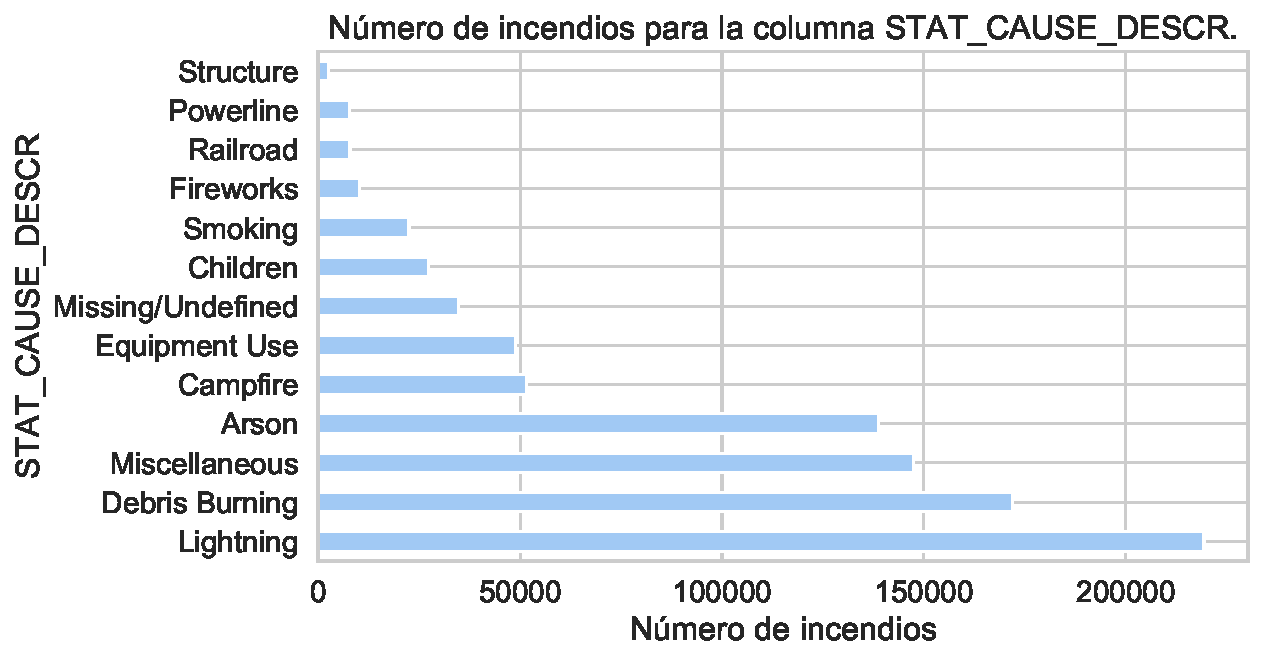
\includegraphics[width=0.48\textwidth]{imagenes/barh_STAT_CAUSE_DESCR.pdf}
    \caption{Gráfico de Causas vs. Número de incendios.}
    \label{fig:SCD}
\end{figure}

\section{Análisis Exploratorio de los Datos}\label{EDA}

\subsection{Distribución de las causas de un incendio}
La primera pregunta que alguien se puede realizar es: ¿Cómo están distribuidos el número de incendios con respecto a la causa del incendio? Para responder a la interrogante, se procede a graficar el número de incendios con respecto a sus causas. El resultado del gráfico se puede observar en la Fig.~\ref{fig:SCD}.

Se puede observar que las principales causas de incendio son producidos por rayos (\textit{Lightning}), quema de escombros (\textit{Debris Burning}), de forma miscelánea (\textit{Miscellaneous}) y por razones maliciosas (\textit{Arson}). Mientras que el resto de causas tienen un papel minoritario. 

También, otra de las primeras observaciones que se pueden rescatar, es que el \textit{dataset} se encuentra \textit{desequilibrado} (i.e., que existen clases bastante más númerosas que otras). Esto causará que a la hora de realizar clasificación, las clases con mayor número de incendios (como \textit{Lightning}) queden beneficiadas frente a las clases minoritarias (como \textit{Structure}), resultando en \textit{overfitting}.

Para solucionar este problema, se crearán 4 nuevas categorías, como se explica en \ref{subsec:nuevas-cats}. estas son: \textbf{Natural}, \textbf{Malicious}, \textbf{Other} y \textbf{Human}. En la Fig.~\ref{fig:SCDN} se puede observar la nueva distribución que resulta de la creación de las nuevas categorías.
\begin{figure}
    \centering
    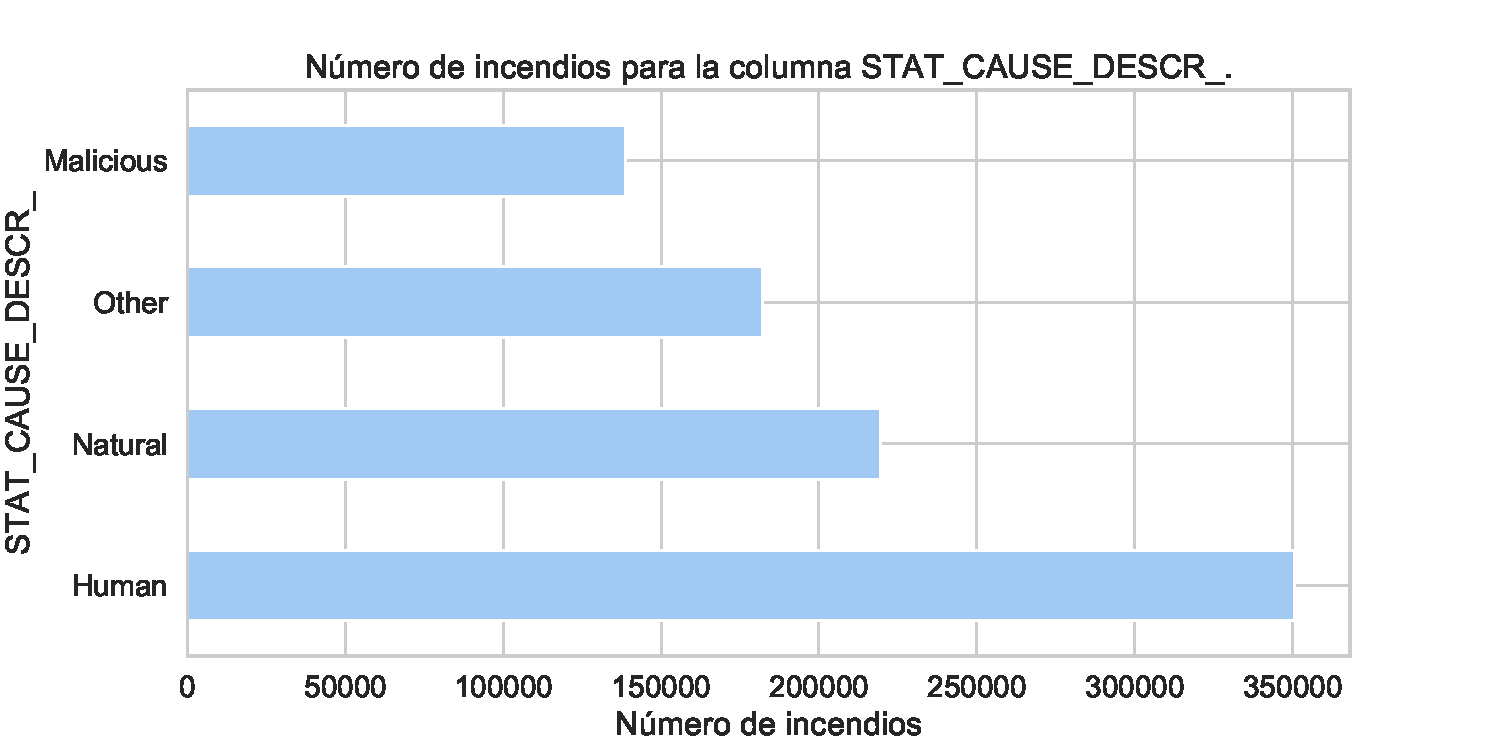
\includegraphics[width=0.48\textwidth]{imagenes/barh_STAT_CAUSE_DESCR_.pdf}
    \caption{Gráfico de Causas Nuevas vs. Número de incendios.}
    \label{fig:SCDN}
\end{figure}

Se puede observar a primera vista que la nueva categorización resulta en un \textit{dataset} más balanceado, y que además, la causa humana resulta ser la nueva clase mayoritaria.

\subsection{Distribución de los incendios a lo largo de los años}
Otra interrogante que se puede plantear es: ¿Cómo se distribuyen los incendios a lo largo de los años? Para responder a esta pregunta, se elaboró un gráfico del número de incendios vs. el año de ocurrencia. El resultado del gráfico se puede observar en la Fig.~\ref{fig:Year-Ocurr}.
\begin{figure}
    \centering
    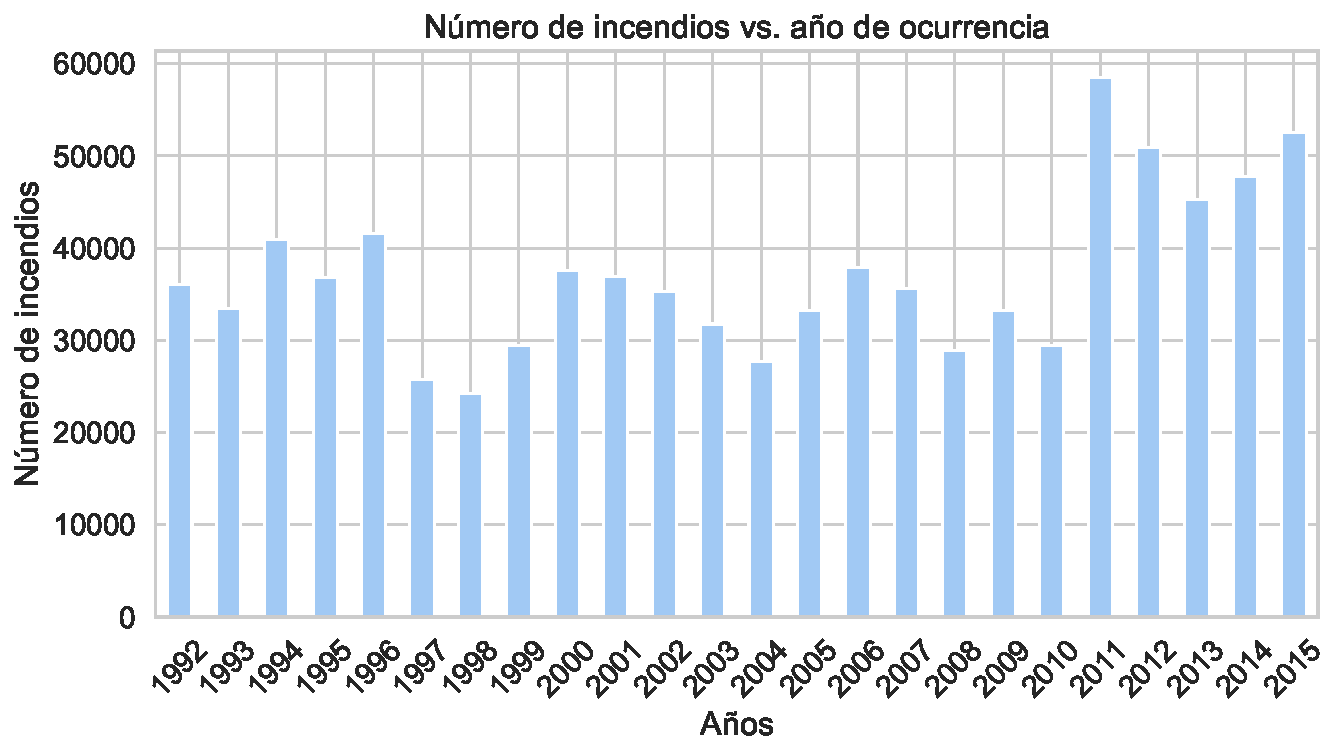
\includegraphics[width=0.48\textwidth]{imagenes/YEAR_OCURRENCIA.pdf}
    \caption{Gráfico de Número de incendios vs. Año de ocurrencia.}
    \label{fig:Year-Ocurr}
\end{figure}

Las primeras apreciaciones que se observan es que en los últimos años (desde el 2011 hasta el 2015) se tuvo un alza importante de incendios. Quizás, esto se puede deber a que en los últimos años se cambió la forma en que se contabilizaban los incendios, o quizás que en esos años ocurrieron incendios con el interés de ocupar el terreno.

Además, también se observa que hay años que son minoría comparativamente, como por ejemplo, en el año 2011 ocurrieron más del doble de incendios que en el año 1998. 

Es importante tomar en cuenta estas observaciones, pues puede afectar en la predicción del clasificador en gran medida, pues este no estará consciente de las ``rachas'' de incendios que ocurrieron en los últimos años.

Luego, una interrogante natural que surge es: ¿Cómo se distribuyen las causas de los incendios a lo largo de los años? Para responder a esta pregunta, se 










% Visualizaciones y resultados relevantes.

% - Análisis exploratorio de datos, mostrar solo visualizaciones y resultados relevantes.
% - Lo realizado para la presentación 1 (que en algunos casos sería lo mismo del análisis exploratorio, o los primeros problemas que tuvieron con sus bases de datos o problemas)
% - Lo realizado para la presentación 2, que sería mostrar en algunos casos el primer experimento que realizaron para resolver su problema, o en otros sería plantear el por qué cambiaron su problema o base de datos.

\section{Metodología}

% - Dado lo encontrado en lo realizado anteriormente, plantear cómo podrían abordar los problemas obtenidos, mejorar métricas, cambios en la metodología, etc.

\subsection{Modelos}
Se propondrá cinco modelos para la clasificación, escogidos en base a los algoritmos vistos en el curso. Estos son: \textit{Naïve Bayes}, \textit{K-Vecinos más Cercanos}, \textit{Discriminante Lineal}, \textit{Discriminante Cuadrático} y \textit{Random Forest}

\subsubsection{Preparación del modelo de Naïve Bayes}
Para el modelo de \textit{Naïve Bayes}, no se seleccionarán hiperparámetros. Se asumirá un prior uniforme, pues de todas formas, se considera que se tienen suficientes datos como para que el prior se vuelva irrelevante. 

\subsubsection{Preparación del modelo de K-NN}
Para el modelo de los \textit{K-Vecinos más Cercanos}, se empezará por normalizar los datos y escogiendo con anterioridad un $k$ óptimo, de forma heurística. 

La metodología para encontrar este $k$ óptimo, es probando con una lista finita de valores tentativos (e.g.: $k\in\{1, 10, 50, 100, 150, 200\}$) y evaluando cuál posee el mayor \textit{score}. Realizado esto, se procede a realizar una nueva iteración en la vecindad en que se encontraba el $k$ anterior (e.g.: si resultó que $k=50$ en el ejemplo anterior, entonces se probará en un conjunto acotado que esté entre $10$ y $100$).

\subsubsection{Preparación del modelo lineal/cuadrático}
No se realizará una preparación previa para estos modelos, ni se ajustarán sus hiperparámetros.

\subsubsection{Preparación del modelo de Random Forest}
Dada a la gran cantidad de datos que posee el dataset, y al gran costo computacional que supone este algoritmo, resulta muy difícil ajustar los hiperparámetros que posee, con lo que se prefiere conservar los hiperparámetros que viene por defecto con el modelo.

% Cabe destacar que la forma en que se encontrará el $k$ óptimo para el algoritmo de \textit{KNN} será de manera Heurística, es decir, se probará primero con un conjunto de tentativo para los $k$, y se escogerá el $k$ de forma que maximice la puntuación de este clasificador. Mientras que los hiperparámetros del \textit{Random Forest} serán los que viene por defecto en la librería de \textit{sklearn}.

% \subsection{Validación}

\subsection{Escenarios}
Se propondrá distintos escenarios en los que se aplicarán los cinco modelos descritos anteriormente.

\subsubsection{Todos los datos}
En este escenario se considerarán todos los datos que contiene el \textit{dataset} posterior a su depuración, sin realizar un ``preprocesamiento''. Se realizará esto para comparar la eficiencia que poseen los otros escenarios frente a ``no realizar nada''.

\subsubsection{A partir del año 2011}

Como se observó en la Fig.~\ref{fig:Year-Ocurr}, ocurre una alza importante en estos años, dando una regularidad significativa frente a los años anteriores. Es por esto que se probarán los distintos modelos en el escenario de los últimos años a partir del 2011.

\subsubsection{Agrupación de las categorías}
Cómo se habló en la sección~\ref{EDA}, existe un desbalance bastante importante en las categorías de las causas de un incendio. Es por esto que se considerará en realizar una recategorización de los datos y además, al igual que en el escenario anterior, se considerarán los últimos años a partir de 2011.

% \subsubsection{}


% Escenario en que no se tocan mucho los datos

% Escenario en que se considera los datos de los últimos años

% Escenario en que se considera los datos del último año y las nuevas categorías

\subsection{Preparación del Conjunto de Entrenamiento y Test}
Dado a que los datos tienen una dependencia temporal, se dividirá un conjunto de entrenamiento y un conjunto de test de forma que, el primer $90\%$ de los datos serán asignados al entrenamiento, y el $10\%$ restantes serán asignados para el test. 

La razón de esta división es que se busca predecir el futuro en base al pasado, y si simplemente se toma una muestra aleatoria del \textit{dataset}, si después se busca predecir una causa, puede ``aprenderse'' la respuesta de antemano para decir la causa. Es más, esta fue una falla que se tuvo en la primera presentación.

% Escenario en que se predicen solo las causas malévolas, o solo las causas humanas.

\section{Resultados y Discusión}
El resumen de las exactitudes (\textit{accuracy}) de cada uno de los modelos frente a cada uno de los escenarios se encuentra en la Tabla~\ref{tab:resumen-exp}.

\begin{table}
\centering
\caption{Tabla resumen de los modelos}
\label{tab:resumen-exp}
\begin{tabular}{rccc}
\toprule
{} &  Experimento 1 &  Experimento 2 &  Experimento 3 \\
Modelos                  &                &                &                \\
\midrule
Naive Bayes              &         0.2215 &         0.1400 &         0.3574 \\
Discriminante Cuadrático &         0.2451 &         0.1512 &         0.3870 \\
Discriminante Lineal     &         0.3465 &         0.3233 &         0.4210 \\
KNN                      &         0.3978 &         0.4266 &         0.5459 \\
Random Forest            &         0.4562 &         0.5277 &         0.6467 \\
\bottomrule
\end{tabular}
\end{table}


A continuación, se presentará un resumen de las distintas métricas que se utilizan para evaluar la eficiencia de una clasificación, para algunos de algunos modelos que tuvieron un buen desempeño en la clasificación de los tres escenarios.

\begin{table}
\centering
\caption{Reporte de clasificación para el Escenario 1 utilizando Discriminante Cuadrático}
\label{tab:DC_Escenario 1}
\begin{tabular}{lrrr}
\toprule
{} &  precision &  recall &  f1-score \\
\midrule
Arson             &      0.201 &   0.110 &     0.142 \\
Campfire          &      0.169 &   0.039 &     0.064 \\
Children          &      0.030 &   0.449 &     0.057 \\
Debris Burning    &      0.405 &   0.705 &     0.514 \\
Equipment Use     &      0.000 &   0.000 &     0.000 \\
Fireworks         &      0.067 &   0.438 &     0.116 \\
Lightning         &      0.565 &   0.220 &     0.316 \\
Miscellaneous     &      0.467 &   0.051 &     0.092 \\
Missing/Undefined &      0.000 &   0.000 &     0.000 \\
Powerline         &      0.000 &   0.000 &     0.000 \\
Railroad          &      0.000 &   0.000 &     0.000 \\
Smoking           &      0.000 &   0.000 &     0.000 \\
Structure         &      0.033 &   0.014 &     0.020 \\
accuracy          &            &         &     0.245 \\
macro avg         &      0.149 &   0.156 &     0.102 \\
weighted avg      &      0.319 &   0.245 &     0.217 \\
\bottomrule
\end{tabular}
\end{table}



% \section{Discusión}

% - Discusión, si es que lo requieren, para englobar todos sus experimentos y resultados


\section{Conclusión}

\subsection{Conclusión acerca del Escenario 1}
Podemos observar que en el primer escenario, las predicciones de la mayoría de los modelos son insatisfactorias. Inclusive el modelo de \textit{Random Forest}, que posee un $45.6\%$ de exactitud, es un porcentaje relativamente bajo. 

Esto se puede deber a que el modelo se aprendió ciertos patrones del pasado (digamos, de los años 1992 a 2010) para después ver que en los años futuros, todo el escenario cambió radicalmente, como se puede observar en la Fig.~\ref{fig:Year-Ocurr}.

Además, de las Tablas \ref{tab:RF_Escenario 1} hasta la \ref{tab:NB_Escenario 1}, se observa que por lo usual, la causa \textbf{Lightning} es la que posee mayor \textit{recall}. Es lo esperable, pues es la causa con mayor número de incendios, y para los modelos le resulta más fácil decir que pertenece a la clase mayoritaria que a las clases minoritarias. A fin de cuentas, este Escenario sufre de un \textit{overfitting}.

\subsection{Conclusión acerca del Escenario 2}


\subsection{Conclusión acerca del Escenario 3}

\begin{thebibliography}{00}
\bibitem{FPA} Short, Karen C. 2017. Spatial wildfire occurrence data for the United States, 1992-2015 [FPA\_FOD\_20170508]. 4th Edition. Fort Collins, CO: Forest Service Research Data Archive. \url{https://doi.org/10.2737/RDS-2013-0009.4}

% \bibitem{b1} G. Eason, B. Noble, and I. N. Sneddon, ``On certain integrals of Lipschitz-Hankel type involving products of Bessel functions,'' Phil. Trans. Roy. Soc. London, vol. A247, pp. 529--551, April 1955.
% \bibitem{b2} J. Clerk Maxwell, A Treatise on Electricity and Magnetism, 3rd ed., vol. 2. Oxford: Clarendon, 1892, pp.68--73.
% \bibitem{b3} I. S. Jacobs and C. P. Bean, ``Fine particles, thin films and exchange anisotropy,'' in Magnetism, vol. III, G. T. Rado and H. Suhl, Eds. New York: Academic, 1963, pp. 271--350.
% \bibitem{b4} K. Elissa, ``Title of paper if known,'' unpublished.
% \bibitem{b5} R. Nicole, ``Title of paper with only first word capitalized,'' J. Name Stand. Abbrev., in press.
% \bibitem{b6} Y. Yorozu, M. Hirano, K. Oka, and Y. Tagawa, ``Electron spectroscopy studies on magneto-optical media and plastic substrate interface,'' IEEE Transl. J. Magn. Japan, vol. 2, pp. 740--741, August 1987 [Digests 9th Annual Conf. Magnetics Japan, p. 301, 1982].
% \bibitem{b7} M. Young, The Technical Writer's Handbook. Mill Valley, CA: University Science, 1989.
\end{thebibliography}
\newpage

\appendices
\section{Reportes de Clasificación}\label{append:rep-clasf}
A continuación se presentarán los distintos reportes de clasificación por cada modelo y por cada escenario descrito:
\subsection{Escenario 1}\label{append:escn1}
Los resultados de la clasificación en el Escenario 1 utilizando \textit{Random Forest}, \textit{K-Vecinos más cercanos}, \textit{Discriminante lineal}, \textit{Discriminante Cuadrático} y \textit{Naïve Bayes} se encuentran en las Tablas \ref{tab:RF_Escenario 1}, \ref{tab:KNN_Escenario 1}, \ref{tab:DL_Escenario 1}, \ref{tab:DC_Escenario 1} y \ref{tab:NB_Escenario 1} respectivamente. 

\subsection{Escenario 2}\label{append:escn2}
Los resultados de la clasificación en el Escenario 2 utilizando \textit{Random Forest}, \textit{K-Vecinos más cercanos}, \textit{Discriminante lineal}, \textit{Discriminante Cuadrático} y \textit{Naïve Bayes} se encuentran en las Tablas \ref{tab:RF_Escenario 2}, \ref{tab:KNN_Escenario 2}, \ref{tab:DL_Escenario 2}, \ref{tab:DC_Escenario 2} y \ref{tab:NB_Escenario 2} respectivamente. 

\subsection{Escenario 3}\label{append:escn3}
Los resultados de la clasificación en el Escenario 3 utilizando \textit{Random Forest}, \textit{K-Vecinos más cercanos}, \textit{Discriminante lineal}, \textit{Discriminante Cuadrático} y \textit{Naïve Bayes} se encuentran en las Tablas \ref{tab:RF_Escenario 3}, \ref{tab:KNN_Escenario 3}, \ref{tab:DL_Escenario 3}, \ref{tab:DC_Escenario 3} y \ref{tab:NB_Escenario 3} respectivamente. 

\newpage
\begin{table}
\centering
\caption{Reporte de clasificación para el Escenario 1 utilizando Random Forest}
\label{tab:RF_Escenario 1}
\begin{tabular}{lrrr}
\toprule
{} &  precision &  recall &  f1-score \\
\midrule
Arson             &      0.283 &   0.358 &     0.316 \\
Campfire          &      0.348 &   0.251 &     0.291 \\
Children          &      0.236 &   0.110 &     0.150 \\
Debris Burning    &      0.537 &   0.584 &     0.560 \\
Equipment Use     &      0.236 &   0.133 &     0.170 \\
Fireworks         &      0.510 &   0.308 &     0.384 \\
Lightning         &      0.650 &   0.839 &     0.733 \\
Miscellaneous     &      0.394 &   0.459 &     0.424 \\
Missing/Undefined &      0.239 &   0.160 &     0.192 \\
Powerline         &      0.102 &   0.004 &     0.008 \\
Railroad          &      0.128 &   0.017 &     0.031 \\
Smoking           &      0.138 &   0.022 &     0.037 \\
Structure         &      0.258 &   0.019 &     0.035 \\
accuracy          &            &         &     0.456 \\
macro avg         &      0.312 &   0.251 &     0.256 \\
weighted avg      &      0.421 &   0.456 &     0.430 \\
\bottomrule
\end{tabular}
\end{table}

\begin{table}
\centering
\caption{KNN_Escenario 1}
\label{tab:Reporte de clasificación para el Escenario 1 utilizando KNN}
\begin{tabular}{lrrr}
\toprule
{} &  precision &  recall &  f1-score \\
\midrule
Arson             &      0.217 &   0.318 &     0.258 \\
Campfire          &      0.183 &   0.113 &     0.140 \\
Children          &      0.187 &   0.078 &     0.110 \\
Debris Burning    &      0.479 &   0.553 &     0.513 \\
Equipment Use     &      0.187 &   0.047 &     0.074 \\
Fireworks         &      0.346 &   0.233 &     0.279 \\
Lightning         &      0.524 &   0.822 &     0.640 \\
Miscellaneous     &      0.372 &   0.379 &     0.375 \\
Missing/Undefined &      0.003 &   0.001 &     0.002 \\
Powerline         &      0.222 &   0.001 &     0.003 \\
Railroad          &      0.035 &   0.005 &     0.008 \\
Smoking           &      0.000 &   0.000 &     0.000 \\
Structure         &      0.000 &   0.000 &     0.000 \\
accuracy          &            &         &     0.398 \\
macro avg         &      0.212 &   0.196 &     0.185 \\
weighted avg      &      0.338 &   0.398 &     0.354 \\
\bottomrule
\end{tabular}
\end{table}

\begin{table}
\centering
\caption{Reporte de clasificación para el Escenario 1 utilizando Discriminante Lineal}
\label{tab:DL_Escenario 1}
\begin{tabular}{lrrr}
\toprule
{} &  precision &  recall &  f1-score \\
\midrule
Arson             &      0.280 &   0.082 &     0.126 \\
Campfire          &      0.026 &   0.000 &     0.000 \\
Children          &      0.000 &   0.000 &     0.000 \\
Debris Burning    &      0.389 &   0.658 &     0.489 \\
Equipment Use     &      0.000 &   0.000 &     0.000 \\
Fireworks         &      0.000 &   0.000 &     0.000 \\
Lightning         &      0.334 &   0.811 &     0.473 \\
Miscellaneous     &      0.280 &   0.201 &     0.234 \\
Missing/Undefined &      0.000 &   0.000 &     0.000 \\
Powerline         &      0.000 &   0.000 &     0.000 \\
Railroad          &      0.000 &   0.000 &     0.000 \\
Smoking           &      0.000 &   0.000 &     0.000 \\
Structure         &      0.000 &   0.000 &     0.000 \\
accuracy          &            &         &     0.346 \\
macro avg         &      0.101 &   0.135 &     0.102 \\
weighted avg      &      0.237 &   0.346 &     0.258 \\
\bottomrule
\end{tabular}
\end{table}

\begin{table}
\centering
\caption{Reporte de clasificación para el Escenario 1 utilizando Discriminante Cuadrático}
\label{tab:DC_Escenario 1}
\begin{tabular}{lrrr}
\toprule
{} &  precision &  recall &  f1-score \\
\midrule
Arson             &      0.201 &   0.110 &     0.142 \\
Campfire          &      0.169 &   0.039 &     0.064 \\
Children          &      0.030 &   0.449 &     0.057 \\
Debris Burning    &      0.405 &   0.705 &     0.514 \\
Equipment Use     &      0.000 &   0.000 &     0.000 \\
Fireworks         &      0.067 &   0.438 &     0.116 \\
Lightning         &      0.565 &   0.220 &     0.316 \\
Miscellaneous     &      0.467 &   0.051 &     0.092 \\
Missing/Undefined &      0.000 &   0.000 &     0.000 \\
Powerline         &      0.000 &   0.000 &     0.000 \\
Railroad          &      0.000 &   0.000 &     0.000 \\
Smoking           &      0.000 &   0.000 &     0.000 \\
Structure         &      0.033 &   0.014 &     0.020 \\
accuracy          &            &         &     0.245 \\
macro avg         &      0.149 &   0.156 &     0.102 \\
weighted avg      &      0.319 &   0.245 &     0.217 \\
\bottomrule
\end{tabular}
\end{table}

\begin{table}
\centering
\caption{NB_Escenario 1}
\label{tab:Reporte de clasificación para el Escenario 1 utilizando Naïve Bayes}
\begin{tabular}{lrrr}
\toprule
{} &  precision &  recall &  f1-score \\
\midrule
Arson             &      0.185 &   0.103 &     0.132 \\
Campfire          &      0.097 &   0.068 &     0.080 \\
Children          &      0.033 &   0.422 &     0.061 \\
Debris Burning    &      0.371 &   0.706 &     0.486 \\
Equipment Use     &      0.000 &   0.000 &     0.000 \\
Fireworks         &      0.066 &   0.540 &     0.118 \\
Lightning         &      0.500 &   0.087 &     0.148 \\
Miscellaneous     &      0.433 &   0.041 &     0.076 \\
Missing/Undefined &      0.333 &   0.000 &     0.000 \\
Powerline         &      0.000 &   0.000 &     0.000 \\
Railroad          &      0.000 &   0.000 &     0.000 \\
Smoking           &      0.000 &   0.000 &     0.000 \\
Structure         &      0.037 &   0.028 &     0.032 \\
accuracy          &            &         &     0.221 \\
macro avg         &      0.158 &   0.153 &     0.087 \\
weighted avg      &      0.312 &   0.221 &     0.177 \\
\bottomrule
\end{tabular}
\end{table}

% \newpage

% \subsection{Escenario 2}\label{append:escn2}
% Los resultados de la clasificación en el escenario 2 utilizando \textit{Random Forest}, \textit{K-Vecinos más cercanos}, \textit{Discriminante lineal}, \textit{Discriminante Cuadrático} y \textit{Naïve Bayes} se encuentran en las Tablas \ref{tab:RF_Escenario 2}, \ref{tab:KNN_Escenario 2}, \ref{tab:DL_Escenario 2}, \ref{tab:DC_Escenario 2} y \ref{tab:NB_Escenario 2} respectivamente. 
\begin{table}
\centering
\caption{RF_Escenario 2}
\label{tab:Reporte de clasificación para el Escenario 2 utilizando Random Forest}
\begin{tabular}{lrrr}
\toprule
{} &  precision &  recall &  f1-score \\
\midrule
Arson             &      0.419 &   0.359 &     0.386 \\
Campfire          &      0.377 &   0.340 &     0.358 \\
Children          &      0.194 &   0.071 &     0.104 \\
Debris Burning    &      0.453 &   0.580 &     0.509 \\
Equipment Use     &      0.327 &   0.133 &     0.189 \\
Fireworks         &      0.592 &   0.360 &     0.448 \\
Lightning         &      0.704 &   0.835 &     0.764 \\
Miscellaneous     &      0.458 &   0.532 &     0.492 \\
Missing/Undefined &      0.566 &   0.552 &     0.559 \\
Powerline         &      0.091 &   0.007 &     0.013 \\
Railroad          &      0.517 &   0.161 &     0.246 \\
Smoking           &      0.301 &   0.042 &     0.073 \\
Structure         &      0.200 &   0.017 &     0.031 \\
accuracy          &            &         &     0.528 \\
macro avg         &      0.400 &   0.307 &     0.321 \\
weighted avg      &      0.499 &   0.528 &     0.502 \\
\bottomrule
\end{tabular}
\end{table}

\begin{table}
\centering
\caption{Reporte de clasificación para el Escenario 2 utilizando KNN}
\label{tab:KNN_Escenario 2}
\begin{tabular}{lrrr}
\toprule
{} &  precision &  recall &  f1-score \\
\midrule
Arson             &      0.329 &   0.251 &     0.285 \\
Campfire          &      0.200 &   0.112 &     0.144 \\
Children          &      0.000 &   0.000 &     0.000 \\
Debris Burning    &      0.342 &   0.576 &     0.429 \\
Equipment Use     &      0.278 &   0.057 &     0.095 \\
Fireworks         &      0.345 &   0.203 &     0.256 \\
Lightning         &      0.553 &   0.803 &     0.655 \\
Miscellaneous     &      0.424 &   0.418 &     0.421 \\
Missing/Undefined &      0.293 &   0.180 &     0.223 \\
Powerline         &      0.154 &   0.004 &     0.009 \\
Railroad          &      0.000 &   0.000 &     0.000 \\
Smoking           &      0.000 &   0.000 &     0.000 \\
Structure         &      0.000 &   0.000 &     0.000 \\
accuracy          &            &         &     0.427 \\
macro avg         &      0.224 &   0.200 &     0.194 \\
weighted avg      &      0.376 &   0.427 &     0.382 \\
\bottomrule
\end{tabular}
\end{table}

\begin{table}
\centering
\caption{DL_Escenario 2}
\label{tab:Reporte de clasificación para el Escenario 2 utilizando Discriminante Lineal}
\begin{tabular}{lrrr}
\toprule
{} &  precision &  recall &  f1-score \\
\midrule
Arson             &      0.000 &   0.000 &     0.000 \\
Campfire          &      0.000 &   0.000 &     0.000 \\
Children          &      0.000 &   0.000 &     0.000 \\
Debris Burning    &      0.252 &   0.792 &     0.382 \\
Equipment Use     &      0.000 &   0.000 &     0.000 \\
Fireworks         &      0.000 &   0.000 &     0.000 \\
Lightning         &      0.410 &   0.790 &     0.540 \\
Miscellaneous     &      0.191 &   0.059 &     0.090 \\
Missing/Undefined &      0.000 &   0.000 &     0.000 \\
Powerline         &      0.000 &   0.000 &     0.000 \\
Railroad          &      0.000 &   0.000 &     0.000 \\
Smoking           &      0.000 &   0.000 &     0.000 \\
Structure         &      0.000 &   0.000 &     0.000 \\
accuracy          &            &         &     0.323 \\
macro avg         &      0.066 &   0.126 &     0.078 \\
weighted avg      &      0.180 &   0.323 &     0.209 \\
\bottomrule
\end{tabular}
\end{table}

\begin{table}
\centering
\caption{DC_Escenario 2}
\label{tab:Reporte de clasificación para el Escenario 2 utilizando Discriminante Cuadrático}
\begin{tabular}{lrrr}
\toprule
{} &  precision &  recall &  f1-score \\
\midrule
Arson             &      0.173 &   0.036 &     0.059 \\
Campfire          &      0.333 &   0.003 &     0.006 \\
Children          &      0.018 &   0.573 &     0.034 \\
Debris Burning    &      0.271 &   0.729 &     0.395 \\
Equipment Use     &      0.167 &   0.002 &     0.003 \\
Fireworks         &      0.094 &   0.143 &     0.113 \\
Lightning         &      0.595 &   0.102 &     0.174 \\
Miscellaneous     &      0.104 &   0.005 &     0.009 \\
Missing/Undefined &      0.221 &   0.056 &     0.089 \\
Powerline         &      0.000 &   0.000 &     0.000 \\
Railroad          &      0.000 &   0.000 &     0.000 \\
Smoking           &      0.000 &   0.000 &     0.000 \\
Structure         &      0.050 &   0.008 &     0.014 \\
accuracy          &            &         &     0.151 \\
macro avg         &      0.156 &   0.127 &     0.069 \\
weighted avg      &      0.277 &   0.151 &     0.119 \\
\bottomrule
\end{tabular}
\end{table}

\begin{table}
\centering
\caption{Reporte de clasificación para el Escenario 2 utilizando Naïve Bayes}
\label{tab:NB_Escenario 2}
\begin{tabular}{lrrr}
\toprule
{} &  precision &  recall &  f1-score \\
\midrule
Arson             &      0.210 &   0.029 &     0.051 \\
Campfire          &      0.000 &   0.000 &     0.000 \\
Children          &      0.018 &   0.579 &     0.035 \\
Debris Burning    &      0.246 &   0.702 &     0.365 \\
Equipment Use     &      0.154 &   0.003 &     0.006 \\
Fireworks         &      0.092 &   0.168 &     0.119 \\
Lightning         &      0.622 &   0.068 &     0.123 \\
Miscellaneous     &      0.110 &   0.007 &     0.013 \\
Missing/Undefined &      0.219 &   0.063 &     0.098 \\
Powerline         &      0.000 &   0.000 &     0.000 \\
Railroad          &      0.000 &   0.000 &     0.000 \\
Smoking           &      0.000 &   0.000 &     0.000 \\
Structure         &      0.000 &   0.000 &     0.000 \\
accuracy          &            &         &     0.140 \\
macro avg         &      0.129 &   0.125 &     0.062 \\
weighted avg      &      0.266 &   0.140 &     0.103 \\
\bottomrule
\end{tabular}
\end{table}

% \newpage

% \subsection{Escenario 3}\label{append:escn3}
% Los resultados de la clasificación en el escenario 3 utilizando \textit{Random Forest}, \textit{K-Vecinos más cercanos}, \textit{Discriminante lineal}, \textit{Discriminante Cuadrático} y \textit{Naïve Bayes} se encuentran en las Tablas \ref{tab:RF_Escenario 3}, \ref{tab:KNN_Escenario 3}, \ref{tab:DL_Escenario 3}, \ref{tab:DC_Escenario 3} y \ref{tab:NB_Escenario 3} respectivamente. 
\begin{table}
\centering
\caption{RF_Escenario 3}
\label{tab:Reporte de clasificación para el Escenario 3 utilizando Random Forest}
\begin{tabular}{lrrr}
\toprule
{} &  precision &  recall &  f1-score \\
\midrule
Human        &      0.605 &   0.684 &     0.642 \\
Malicious    &      0.554 &   0.280 &     0.372 \\
Natural      &      0.753 &   0.781 &     0.767 \\
Other        &      0.625 &   0.598 &     0.611 \\
accuracy     &            &         &     0.647 \\
macro avg    &      0.634 &   0.586 &     0.598 \\
weighted avg &      0.644 &   0.647 &     0.640 \\
\bottomrule
\end{tabular}
\end{table}

\begin{table}
\centering
\caption{Reporte de clasificación para el Escenario 3 utilizando KNN}
\label{tab:KNN_Escenario 3}
\begin{tabular}{lrrr}
\toprule
{} &  precision &  recall &  f1-score \\
\midrule
Human        &      0.515 &   0.663 &     0.580 \\
Malicious    &      0.434 &   0.116 &     0.183 \\
Natural      &      0.621 &   0.684 &     0.651 \\
Other        &      0.530 &   0.422 &     0.470 \\
accuracy     &            &         &     0.546 \\
macro avg    &      0.525 &   0.471 &     0.471 \\
weighted avg &      0.539 &   0.546 &     0.529 \\
\bottomrule
\end{tabular}
\end{table}

\begin{table}
\centering
\caption{DL_Escenario 3}
\label{tab:Reporte de clasificación para el Escenario 3 utilizando Discriminante Lineal}
\begin{tabular}{lrrr}
\toprule
{} &  precision &  recall &  f1-score \\
\midrule
Human        &      0.414 &   0.772 &     0.539 \\
Malicious    &      0.000 &   0.000 &     0.000 \\
Natural      &      0.437 &   0.569 &     0.494 \\
Other        &      0.389 &   0.026 &     0.050 \\
accuracy     &            &         &     0.421 \\
macro avg    &      0.310 &   0.342 &     0.271 \\
weighted avg &      0.377 &   0.421 &     0.328 \\
\bottomrule
\end{tabular}
\end{table}

\begin{table}
\centering
\caption{DC_Escenario 3}
\label{tab:Reporte de clasificación para el Escenario 3 utilizando Discriminante Cuadrático}
\begin{tabular}{lrrr}
\toprule
{} &  precision &  recall &  f1-score \\
\midrule
Human        &      0.387 &   0.905 &     0.542 \\
Malicious    &      0.160 &   0.123 &     0.139 \\
Natural      &      0.613 &   0.148 &     0.239 \\
Other        &      0.409 &   0.068 &     0.116 \\
accuracy     &            &         &     0.387 \\
macro avg    &      0.392 &   0.311 &     0.259 \\
weighted avg &      0.431 &   0.387 &     0.298 \\
\bottomrule
\end{tabular}
\end{table}

\begin{table}
\centering
\caption{NB_Escenario 3}
\label{tab:Reporte de clasificación para el Escenario 3 utilizando Naïve Bayes}
\begin{tabular}{lrrr}
\toprule
{} &  precision &  recall &  f1-score \\
\midrule
Human        &      0.372 &   0.892 &     0.526 \\
Malicious    &      0.172 &   0.175 &     0.173 \\
Natural      &      0.573 &   0.069 &     0.123 \\
Other        &      0.280 &   0.036 &     0.064 \\
accuracy     &            &         &     0.357 \\
macro avg    &      0.349 &   0.293 &     0.221 \\
weighted avg &      0.376 &   0.357 &     0.250 \\
\bottomrule
\end{tabular}
\end{table}




\end{document}
